\documentclass[11pt,a4paper]{article}
\usepackage[margin=2.2cm]{geometry}
\usepackage[T1]{fontenc}\usepackage{lmodern}
\usepackage{graphicx,booktabs,tabularx,tikz,enumitem,microtype}
\usetikzlibrary{positioning}
\setlist{nosep,leftmargin=1.4em}
\setlength{\parskip}{3pt}\setlength{\parindent}{0pt}
\usepackage[hidelinks]{hyperref}
\usepackage{titlesec}
\titlespacing*{\section}{0pt}{10pt}{4pt}
\titlespacing*{\subsection}{0pt}{6pt}{2pt}
\begin{document}
\begin{center}
{\LARGE\bfseries Nexus: Network Intelligence and Autonomous DevSecOps}\\[4pt]
Aryan Khanna, SIT Pune\\
Incedo Northstars Mini Project (Individual)\\
\url{https://github.com/aryankhanna1409/nexus}
\end{center}

\section{Problem Statement}
When a telecom network degrades, engineers have to work out the cause by hand from call records, KPI counters, recent deployments, configuration changes and security events. This takes time, and the fix often comes late. Nexus automates the chain. It analyses call logs, detects anomalies in network counters, correlates them with recent changes, runs an AI root-cause investigation, writes an incident report, and lets an agent carry out the remediation under a policy gate. Every AI decision and agent action is recorded in an audit log.

All data used in this project is synthetic. The telemetry, call logs, deployments and security events are generated by a simulator, and the production rollback is simulated.

\section{System Architecture}
\begin{center}
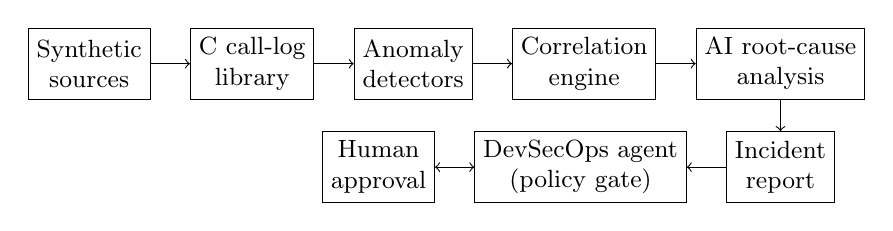
\begin{tikzpicture}[node distance=4mm and 5mm, b/.style={draw,align=center,font=\small,minimum height=9mm,inner sep=3pt}]
\node[b] (s) {Synthetic\\sources};
\node[b,right=of s] (c) {C call-log\\library};
\node[b,right=of c] (d) {Anomaly\\detectors};
\node[b,right=of d] (k) {Correlation\\engine};
\node[b,right=of k] (r) {AI root-cause\\analysis};
\node[b,below=of r] (p) {Incident\\report};
\node[b,left=of p] (a) {DevSecOps agent\\(policy gate)};
\node[b,left=of a] (h) {Human\\approval};
\draw[->] (s)--(c); \draw[->] (c)--(d); \draw[->] (d)--(k); \draw[->] (k)--(r); \draw[->] (r)--(p); \draw[->] (p)--(a); \draw[<->] (a)--(h);
\end{tikzpicture}
\end{center}
The services sit behind a FastAPI REST API with token authentication and four roles: viewer, operator, approver and admin. Storage is PostgreSQL (SQLite for offline runs) and Redis, and the user interface is a React and TypeScript dashboard. The language model layer runs on NVIDIA NIM. OpenAI and Anthropic APIs can be plugged in as optional providers without code changes, and a deterministic mock provider is used for offline runs and tests.

\begin{tabularx}{\linewidth}{@{}llX@{}}
\toprule
Component & Location & Responsibility\\\midrule
Call analyzer & \texttt{c-library/} & Parses and validates CDRs, aggregates per cell, flags outliers (C11)\\
Simulator & \texttt{app/simulation/} & Causal time-series model with injected incidents\\
Analytics & \texttt{app/analytics/} & EWMA, threshold and z-score detectors; correlation into incidents\\
RCA engine & \texttt{app/rca/} & LLM investigation over read-only tools, with schema-validated output\\
Reporting & \texttt{app/reporting/} & JSON, Markdown and HTML incident reports\\
Agent & \texttt{app/agents/} & Observe, analyse, act, verify and close; allowlisted tools with risk classes\\
\bottomrule
\end{tabularx}

\subsection*{Technology stack and mapping to requirements}
\begin{tabularx}{\linewidth}{@{}lXX@{}}
\toprule
Requirement & Technologies & Where in the code\\\midrule
1. Call-log analysis with AI RCA & C11, CMake, ASan/UBSan, Python ctypes, LLM via NVIDIA NIM (OpenAI / Anthropic optional) & \texttt{c-library/}, \texttt{backend/call\_analyzer/}, \texttt{app/rca/}\\
2. AI report on network counters & Python, NumPy, Jinja2, LLM narrative & \texttt{app/analytics/}, \texttt{app/reporting/}\\
3. Autonomous DevSecOps agent & Python state machine, policy engine, role-based approvals, Git & \texttt{app/agents/}\\
Shared platform & FastAPI, PostgreSQL/SQLite, Redis, Alembic, React, TypeScript, Docker Compose, pytest & \texttt{backend/app/api/}, \texttt{frontend/}\\
\bottomrule
\end{tabularx}

\section{Implementation of the Objectives}
\subsection{C library for call-log analysis with AI root-cause investigation}
\texttt{libcallanalyzer} is written in C11 and tested under AddressSanitizer and UndefinedBehaviorSanitizer. It reads the call detail records, computes success, drop and setup-failure rates for each cell, and reports cells that stand out from their peers. Python calls it through ctypes. Its results go to the root-cause engine, where the language model investigates using tools that query metrics, the incident timeline, deployments and call statistics. Each finding in the verdict cites the tool call it came from, and alternative explanations are scored and rejected explicitly.

\subsection{AI report on network counter analytics and anomalies}
The detectors compare latency, jitter, packet loss, CPU, memory, throughput and call drop rate against a rolling baseline. The report combines figures computed directly from stored telemetry with a written narrative from the language model, covering the summary, KPI analysis, timeline and root cause.

\subsection{Autonomous DevSecOps agent}
The agent opens the incident, requests a root-cause analysis, inspects the affected deployment and proposes a fix. Each tool has a risk class: read-only, low-risk or high-risk. A high-risk action such as a production rollback needs approval from an approver and must then be executed by an admin. If anyone tries to execute it before approval, the API rejects the request with HTTP 409. The agent can also run without a human in the loop for actions the policy allows, planning with the model served through NVIDIA NIM.

\section{Test Scenario and Results}
In the test scenario, version 2.4.1 of the packet gateway is deployed to node pgw-1 at 14:05 and leaks memory. Memory rises first, followed by CPU, latency, jitter and call drops on cells 101 to 104. The system detected the incident and attributed it to the deployment with 85\% confidence after 12 tool calls. Once the rollback was approved and executed, the metrics returned to baseline.

\begin{figure}[h]\centering
\includegraphics[width=.49\linewidth]{network.png}\hfill
\includegraphics[width=.49\linewidth]{rca.png}\\[2pt]
\includegraphics[width=.49\linewidth]{agent.png}\hfill
\includegraphics[width=.49\linewidth]{dashboard.png}
\caption{Dashboard views. Top: KPI telemetry and the root-cause verdict. Bottom: agent actions after approval, and network health after recovery.}
\end{figure}

\begin{tabularx}{\linewidth}{@{}lX@{}}
\toprule
Check & Result\\\midrule
End-to-end demo (offline) & Passes in about 8 seconds\\
Root cause & Packet gateway 2.4.1 deployment, 85\% confidence\\
Recovery (last 30 min vs.\ baseline) & Memory 57.8 vs.\ 57.1\%; latency 23.2 vs.\ 22.3 ms; drop rate 0.77 vs.\ 0.77\%\\
Policy gate & Execution before approval rejected (HTTP 409)\\
Audit log & Hash chain verified\\
Backend tests & 360 passed, 3 skipped (need a live Redis)\\
C library tests & All passed, including the sanitizer build\\
\bottomrule
\end{tabularx}

\section{Limitations and Future Work}
\begin{itemize}
\item The data is synthetic. Replaying anonymised real CDRs and counters would be the next step.
\item The rollback is simulated. A real deployment would call Kubernetes or Argo behind the same policy gate.
\item The detectors are statistical. Seasonal or learned baselines would reduce false positives on real traffic.
\end{itemize}

\section{Running the Project}
\texttt{make demo} runs the complete flow offline. \texttt{docker compose up} starts the full stack with the dashboard. Setting \texttt{LLM\_PROVIDER=nim} with an NVIDIA API key switches the system to a real language model; \texttt{openai} or \texttt{anthropic} can be used instead with the matching key.
\end{document}
